\documentclass[aspectratio=169]{beamer}

\usepackage{basileabeam}
\usepackage[most]{tcolorbox}
\usepackage{subcaption}
\usepackage{pgfplots} 


\setbeamercovered{invisible}
\addbibresource{presentation.bib}
% Notes:
%\pgfpagesuselayout{2 on 1}[a4paper,border shrink=5mm]
%\setbeamertemplate{note page}[plain]
%\setbeameroption{show notes on second screen=bottom}

\title              {Graph Denoising for Molecular Imaging}

\author     		{Cédric Mendelin}
\email				{cedric.mendelin@stud.unibas.ch}
\institute          {Department of Mathematics and Computer Science, University of Basel}

\date               {29.06.2022}

\ulogo        		{Template/header}
\ulistelement    	{Template/listelement}

\graphicspath{{Figures/}}

% Options:
%\totalNoSlidesDisabled % To turn off the total number of slides in the footer. Comment this if you want the total number of slides in the footer

%\headerSectionsDisabled % Comment this if you want a fancy header containing your sections.


\newcommand{\norm}[1]{\left\lVert#1\right\rVert}

\begin{document}

\AtBeginSection[]{%
  \frame<beamer>{ 
    \frametitle{Outline}   
    \tableofcontents[currentsection] 
  }
}

\begin{frame}[t,plain]
    \titlepage
\end{frame}

\begin{frame}[t]{Outline}
    \tableofcontents
\end{frame}


%% Presentation content

\chapter{Imaging methods}
\label{sec:imaging}

In the current chapter, imaging methods \textit{computed tomography} and 
\textit{cryo-electron microscopy} (cryo-EM) will be introduced. 
Further, their observation model is defined in a mathematically way and their reconstruction is observed.
Application of cryo-EM is the major motivation for the Master Thesis, 
as the problem is not easy to solve due to dealing with enormous noise and other difficulties.


\section{Computed tomography}
Computed tomography is a well established imaging method.
Using X-ray source, fan shaped beams are produced which scan the imaging object,
resulting in many measurements taken over straight lines \cite{computedTomography}.

\paragraph{Tomography reconstruction:}
Tomographic reconstruction\cite{tomographicReconstruction} is a popular inverse problem. 
The aim is to reconstruct an imaged object from observed measurements.
The reconstruction object can be in two-dimension (2D) or in three-dimension (3D). 

\begin{tcolorbox}[colback=red!5!white,colframe=red!75!black]
    In the Master Thesis, the focus on computed tomography will be on 2D case, which is called \textit{classical tomography reconstruction}.
\end{tcolorbox}

\paragraph{2D tomographic reconstruction:}

Mathematically, the observed measurements can be defined as follows:

\begin{equation}
    \label{eq:2Dreconstruction}
    \begin{aligned}
        y_i[j] &= R(x, \theta_i, s_j) + \eta_i[j] , \text{ with } 1 \leq i \leq N \text{ and } 1 \leq j \leq M,
    \end{aligned}
\end{equation}

where $N$ is number of observations and $M$ the observation dimension.
Then, $x \in L^2(\Omega)$ is the original object with $\Omega \subset \mathbb{R}^2 $ and $L^2$ the Lebesgue space.
Further, $y_i \in \mathbb{R}^M$ is the $i$-th observation with $y_i[j] \in \mathbb{R}$ $j$-th element of the observation.

$R(\cdot; \theta, s): L^2(\Omega) \to L^2(\tilde{\Omega}) , x \mapsto R(x; \theta,s)$ refers to the Radon Transform\cite{radonTransform} 
with $\tilde{\Omega} \subset \mathbb{R}$, $\theta$ as the observation angle from the x-axis and $s_j$ as the sampling point.
$\eta$ refers to noise and is defined as $\eta_i[j] \sim \mathcal{N}(0,\sigma^2)$.

\subparagraph{Filter Backprojection:}
Filter Backprojection \cite{tomographicReconstruction} is a reconstruction method, typically used in classical tomography.
It allows to inverse the Radon Transform and enables reconstruction of the original object $x$. 
The algorithm fails when working with noisy data \cite{cryoEmMath2}.

\section{Cryo-EM}
Cryo-EM is another imaging method, that enables the view of molecules in near-atomic resolution.
In the Master Thesis, only single-particle cryo-EM\cite{singleParticleCryoEm} is considered, when writing about cryo-EM it always refer to single-particle cryo-EM.
During imaging process molecules are frozen in a thin layer of ice, where they are randomly oriented and positioned. 
Random orientation and positioning of molecules makes reconstruction challenging but
the freezing process allows to observe molecules in a stable state where they are not moving.
With an electron microscope, two-dimensional tomographic projection images of the molecules are observed in the ice,
which are called \textit{micrograph}. The frozen molecules are fragile and the electron microscope needs to work with
very low power (electron dose), resulting in highly noisy images. The resulting signal-to-noise ration (SNR)
is typically smaller than 1, which indicates that there is more noise than signal \cite{cryoEmMath2}.
Further, observed molecules are not equal in the sense that there are some structural varieties between
the molecules within a observation.


\paragraph{3D cryo-EM reconstruction:}
Similar to tomographic reconstruction, cryo-EM reconstruction problem \cite{cryoEmMath} is defined.
It can be seen as a 3D reconstruction problem as the original object $x \in L^2(\Omega)$ to be reconstructed is in 3D.
To keep the notation from previous section, now $\Omega \subset \mathbb{R}^3 $ and $\tilde{\Omega} \subset \mathbb{R}^2 $.

Mathematically, the observed measurements can be defined as follows:
\begin{equation}
    \label{eq:cryoEmSimple}
    y_i = \Pi_z ( Rot (x; \theta_i)) + \eta_i, \text{ with } 1 \leq i \leq N
\end{equation}

where $\Pi : L^2(\Omega) \to L^2(\tilde{\Omega}), x \mapsto  \int x(\cdot,\cdot,z) dz$ is the projection operator
and 

$Rot : L^2(\Omega) \to L^2(\Omega), Rot_\theta(x) = \left((x_1,x_2,x_3) \mapsto x( x_1R^1, x_2R^2, x_3R^3)\right)$ is the rotation operator modelling the rotation during freezing.
Further, $\theta_i = [\theta_i^1, \theta_i^2, \theta_i^3 ] $ where entries $ \theta_i^1, \theta_i^2, \theta_i^3 \in \mathbb{R}$ and 
$R = [R^1, R^2, R^3] \in SO(3)$. $\eta_i[j,k] \sim \mathcal{N}(0,\sigma^2I)$ corresponds again to the noise of the observation.


As $y_i$ is not observable directly, discretization is needed:
\begin{equation}
    \label{eq:cryoEmSimpleDiscrete}
    \begin{aligned}
        y_i &= \left( \Pi_z ( Rot (x; \theta_i)) + \eta_i\right)(\Delta), \text{ with } 1 \leq i \leq N \\
        y_i[j,k] &= \Pi_z ( Rot(x; \theta_i))_{j,k} + \eta_i[j,k], \text{ with } 1 \leq i \leq N \text{ and } 1 \leq j,k \leq M    
    \end{aligned}
\end{equation}

where $\Delta \subset \tilde{\Omega}^{M^2}$ is the sampling grid and $M$ is the first and second dimension of the sampling grid.


\subparagraph{Extended formula:} 
Equation~\ref{eg:cryoEmSimple} is a simplified version of cryo-EM.
First of all, point spread function (PSF) of the microscope is not taken into account.
Secondly, structural variety is not taken into account, the underlying object $x$ is not the same 
for every observation as modelled in the equation. 
Precisely, it can be seen as a random signal from an unknown distribution defined over all possible molecules structures.

The equation can be extended and defined as the following:
\begin{equation}
    \label{eq:cryoEmExtended}
    y_i = h_i \circ \Pi_z ( Rot (x_i; \theta_i)) + \eta_i, \text{ with } 1 \leq i \leq N
\end{equation}

where $h_i$ is the PSF of the microscope and $\circ$ defines the convolution.


\begin{tcolorbox}[colback=red!5!white,colframe=red!75!black]
    During Master Thesis, equation~\ref{eq:cryoEmSimpleDiscrete} is used, not the extended version.
\end{tcolorbox}


\subparagraph{Difference to tomographic reconstruction:}
The two problems are highly related, but the cryo-EM reconstruct is more challenging.
During CT observation, the patient is asked to not move and therefore, the angles of projection are known.
Whereas, in cryo-EM this information will be lost during the freezing process.
Secondly, the high level of noise makes cryo-EM much more challenging regarding tomographic reconstruction.


\section{Abstract form}
As the tomographic reconstruction and the cryo-EM reconstruction are rather similar, 
the aim of the Master Thesis will be to design an algorithm, that can be applied in both scenarios.

Therefore, an abstract form of the problems will be defined in the following.
First of all, a similar notation as before is used, but in a more general way
$x \in L^2(\Omega)$ where $\Omega \subset \mathbb{R}^D$ with $D$ as the dimension of the space
and $\tilde{\Omega} \subset \mathbb{R}^{D-1}$.


\begin{equation}
    \begin{aligned}
        y_i &= \left( A(x, \theta_i) + \eta_i \right) (\Delta)\\
    \end{aligned}
\end{equation}

where $y_i \in \tilde{\Omega}^M$ is the observed measurements, $M$ the measurement dimension, $x \in L^2(\Omega)$ our original object, $A$ a non-linear operator 
$A: L^2(\Omega) \to L^2(\tilde{\Omega}), x \mapsto A(x; \theta)$ and

$\eta \sim \mathcal{N}(O, \sigma^2 I)$ gaussian noise. $\Delta \subset \tilde{Omega}^{M^2}$ is a term for discretization.

\paragraph{Classical tomography reconstruction:}

For classical tomography parameters are defined defined with $D=2$ and $\theta \in \mathbb{R}$.
Further, $A(\cdot)$ is the Radon Transform, defined in equation~\ref{eq:2Dreconstruction}.
A distance measure between measurements can be set up by using the $\ell2$-norm $\norm{y_i - y_j}$.

\paragraph{Cryo-Em reconstruction:}
For cryo-EM parameters are defined with $D=3$ and $\theta \in \mathbb{R}^3$.
Further, $A(\cdot)$ can be defined as $\Pi_z \left( Rot(x; \theta) \right)$ 
where $Rot$ is the 3D rotation and $\Pi_z$ the tomographic projection.

As measurements are drawn with some random 3D rotation and projection, 
it can happen that two samples are equivalent up to 2D rotation. 
Consider a first example $y_1$, which has no 3D rotation and 
a second sample $y_2$ with a rotation only in in x-y plane by 45°.
The two samples have a defined in-plane rotation $g$, such that $g y_1 = y_2$.
Therefore, in our distance measure we add this term of in-plan rotation: $min_{g \in SO(1)}\norm{g * y_i - y_j}$, 
which is inspired by the work of \cite{multiDiffusionMaps}. 


\paragraph{High noise regime:}
Cryo-EM measurements are highly noisy, which makes reconstruction challenging. 
There are different ways to reduce noise from measurements, most of them are related to averaging. 
Averaging need to consider similar measurements and ignore diverse ones. 
In the defined abstract model, averaging over paired measurements from $\theta$ should be a good averaging model.
But how can it be achieved? 

One idea would be to measure distances between observation (therefore introduced above).
Another way is to find a low-dimensional embedding which maps our measurements $y$ to some $\theta$.
When talking from low-dimensional embeddings, there is no way around Graph Learning, which will be introduced
in the following chapter.

\begin{tcolorbox}[colback=red!5!white,colframe=red!75!black]
    During the Master Thesis, high-noise regime is the domain of interest.
    The main practical application is cryo-EM, where an algorithm for denoising is expected to boost
    quality of the overall 3D-reconstruction. As cryo-EM is a 3D problem, computed tomography will
    be considered as well which allows to test on a corresponding 2D problem.
    The aim of the Master Thesis is to introduce a denoising algorithm, which is able to work well even 
    on highly noisy data, where cryo-EM is major field of interest.
\end{tcolorbox}


\section{Graphs \& Manifolds}

\begin{frame}{Graph - Definitions}

  \begin{block}{Graph Definition}
    A graph is defined as $G = \langle V,E \rangle$, where $V$ is a set of 
    nodes and $E$ is a set of edges. 
  \end{block}

  \pause

  \begin{columns}
    \column{.55\textwidth}

    \begin{block}{Nodes}
      $(n_1, n_2, \dots) \in \mathbb{R}^F$, with $F$ as node feature dimensions.
    \end{block}
  
    \begin{block}{Edges}
      Edges are defined as a set of tuples $(i, j)$, where $i$ and $j$ determine 
      the index of the nodes.
    \end{block}

    \column{.45\textwidth}
    \begin{figure}
      \centering
      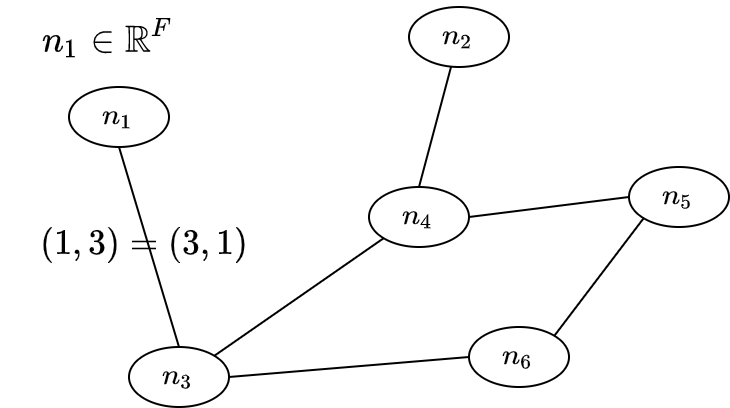
\includegraphics[width=\textwidth]{graph_undirected.drawio.png}
      \caption{Sample graph}        
    \end{figure}
  \end{columns}


  \begin{figure}
    
  \end{figure}

\end{frame}

\begin{frame}{Graph - Definitions - Adjacency Matrix}
\begin{columns}
  \column{.55\textwidth}

  \begin{block}{Adjacency Matrix}
    The binary adjacency matrix of graph $G = \langle V, E \rangle$ is defined as:
  \begin{equation}
      \label{eg:AdjacencyMatrix}
      A_{ij} =    
      \begin{cases}
          1  & \text{if } (i, j) \in E \\
          0, & \text{otherwise}
      \end{cases}
  \end{equation}
  \end{block}

  \pause
  
  \column{.45\textwidth}
  \begin{figure}
    \centering
    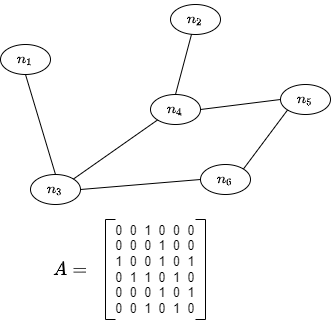
\includegraphics[width=0.9\textwidth]{graph_A.drawio.png}
    \caption{Sample graph}        
  \end{figure}

\end{columns}

\end{frame}

\begin{frame}{Graph - Definitions - Degree}
  \begin{columns}
    \column{.55\textwidth}
  
    \begin{block}{Degree of a node}
      The $degree$ of a node is defined as the number of (incoming) edges.
    \end{block}

    \begin{block}{Degree Matrix of Graph $G$}
      Is a diagonal matrix with degree of nodes as entries.
      $$D_{ii} = degree(n_i)$$
    \end{block}
  
    \pause

    \column{.45\textwidth}
    \begin{figure}
      \centering
      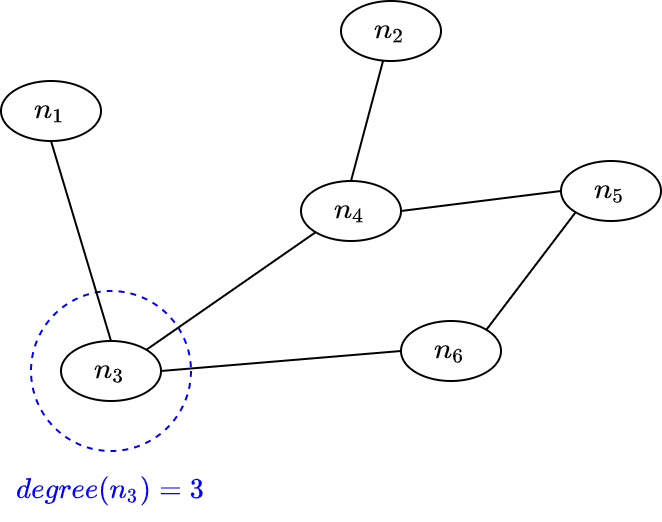
\includegraphics[width=0.9\textwidth]{graph_degree.drawio.png}
      \caption{Sample graph}        
    \end{figure}
  
  \end{columns}
  
  \end{frame}

\begin{frame}{Graph for Molecular Imaging Observation}
  \begin{columns}
    \column{0.45\textwidth}
    \begin{itemize}
      \item Nodes: Single observation $y_i$
      \item Edges: Use k-nearest neighbours (k-NN) to construct a graph
      \item Define similarity measure:
      
    \end{itemize}

    \column{0.55\textwidth}
    \pause
    \begin{figure}
      \centering
      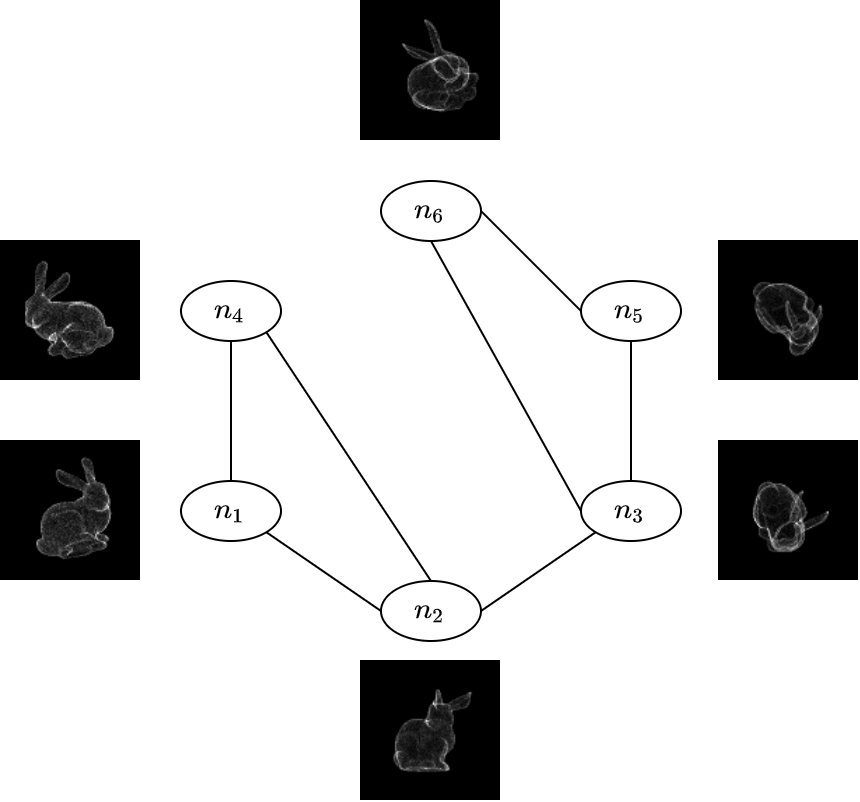
\includegraphics[width=0.8\textwidth]{cryo-EM_graph.drawio.png}
      \caption{Sample graph for cryo-EM observation}        
    \end{figure}
  \end{columns}
\end{frame}

\begin{frame}{Graph for Molecular Imaging Observation - Noise}
  \begin{columns}
    \column{0.45\textwidth}
    \begin{itemize}
      \item With present noise, graph will not capture neighborhood well.
    \end{itemize}

    \column{0.55\textwidth}
    \pause
    \begin{figure}
      \centering
      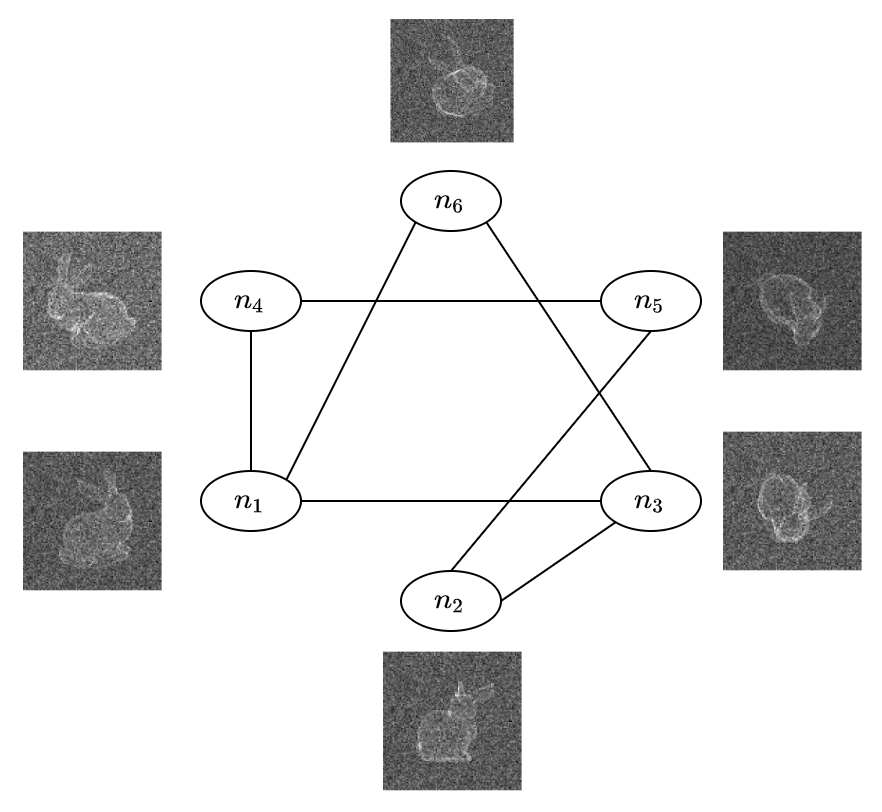
\includegraphics[width=0.8\textwidth]{cryo-EM_graph_noisy.drawio.png}
      \caption{Sample graph for noisy cryo-EM observation}        
    \end{figure}
  \end{columns}
\end{frame}


\begin{frame}{Graph Laplacian (GL)}
\begin{itemize}
  \item What can we use this graph for?
  \item \cite{LaplaceRandomProjections} used it to approximate angles:
\end{itemize}

\begin{block}{Low-dimensional Embedding}
  \begin{enumerate}
    \item Construct a k-NN graph from observations.
    \item Calculate $L = D - A $
    \item Get 2nd and 3rd smallest eigenvalue with corresponding eigenvectors.
  \end{enumerate}
\end{block}

\end{frame}


\begin{frame}{Low-dimensional Embedding for Computed Tomography}
  \begin{figure}
    \centering
    \begin{subfigure}[t]{0.3\textwidth}
        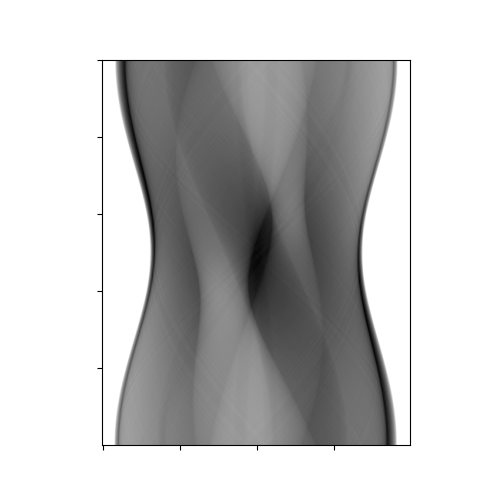
\includegraphics[width=\textwidth]{phantom_sino.png}
        \caption{CT observation}
    \end{subfigure} \hfill
    \begin{subfigure}[t]{0.3\textwidth}
        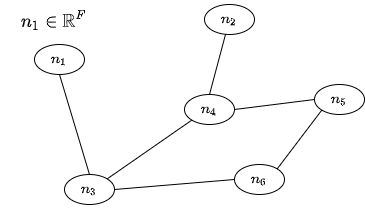
\includegraphics[width=\textwidth]{graph.drawio.png}
        \caption{Building k-NN Graph with $ k = 2$ }
    \end{subfigure}\hfill
    \begin{subfigure}[t]{0.3\textwidth}
      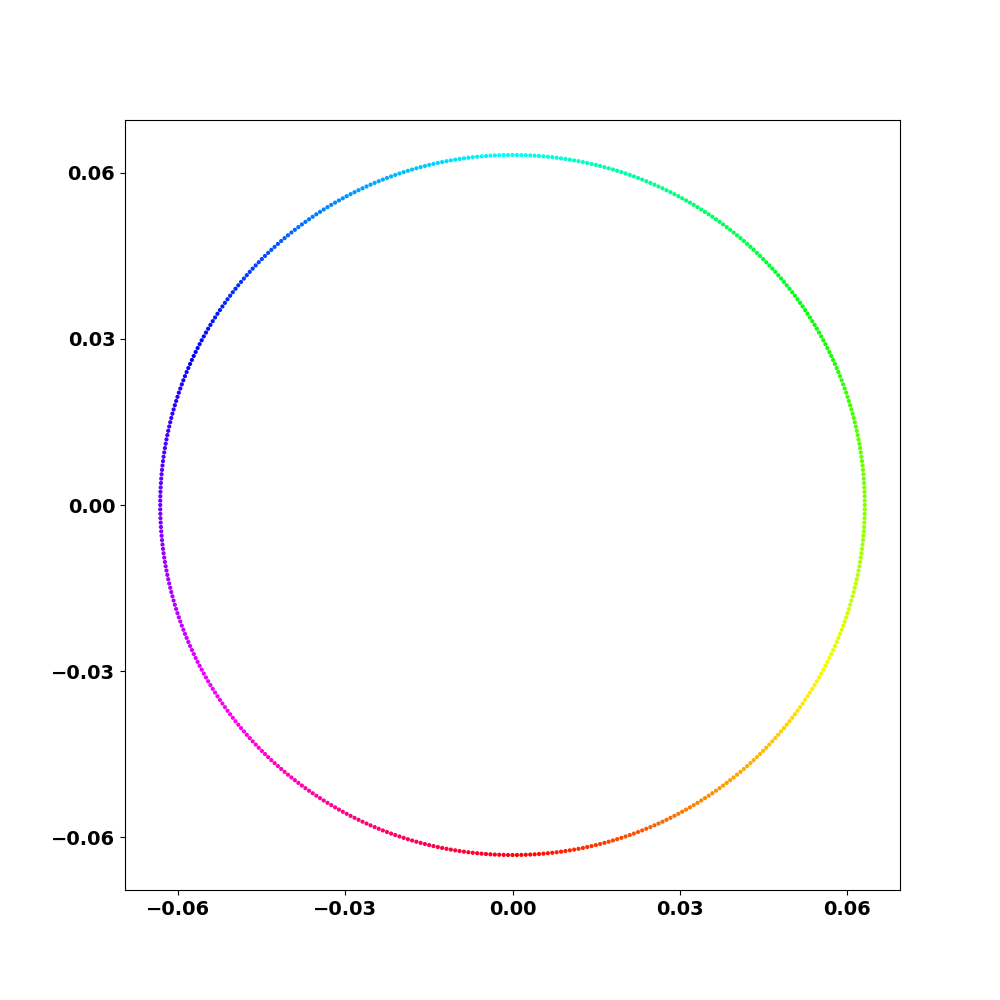
\includegraphics[width=\textwidth]{phaton_clean_manifold.png}
      \caption{$2_{nd}$ and $3_{rd}$ smallest eigenvectors of  $L =  D - A$}
  \end{subfigure}
\end{figure}
  
\end{frame}


\begin{frame}{Computed Tomography with unknown angles}
  \begin{itemize}
    \item GL - Embedding estimated observation angles for noiseless case.
    \item Can be applied for reconstruction.
  \end{itemize}

  \begin{figure}
    \centering
    \only<1-3>{
      \begin{subfigure}[t]{0.3\textwidth}
        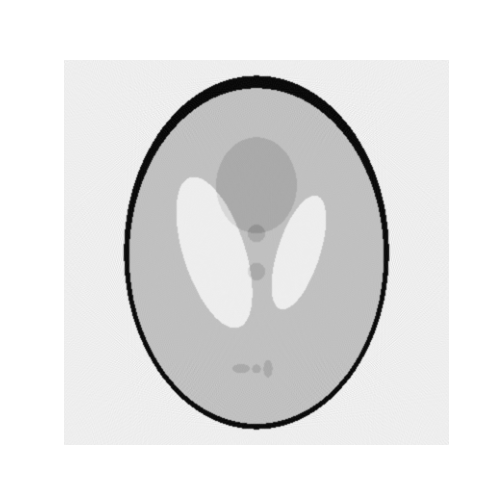
\includegraphics[width=.8\textwidth]{fbp_phantom_clean.png}
        \caption{Reconstruction known angles}
      \end{subfigure} \hfill
      \pause
      \begin{subfigure}[t]{0.3\textwidth}
          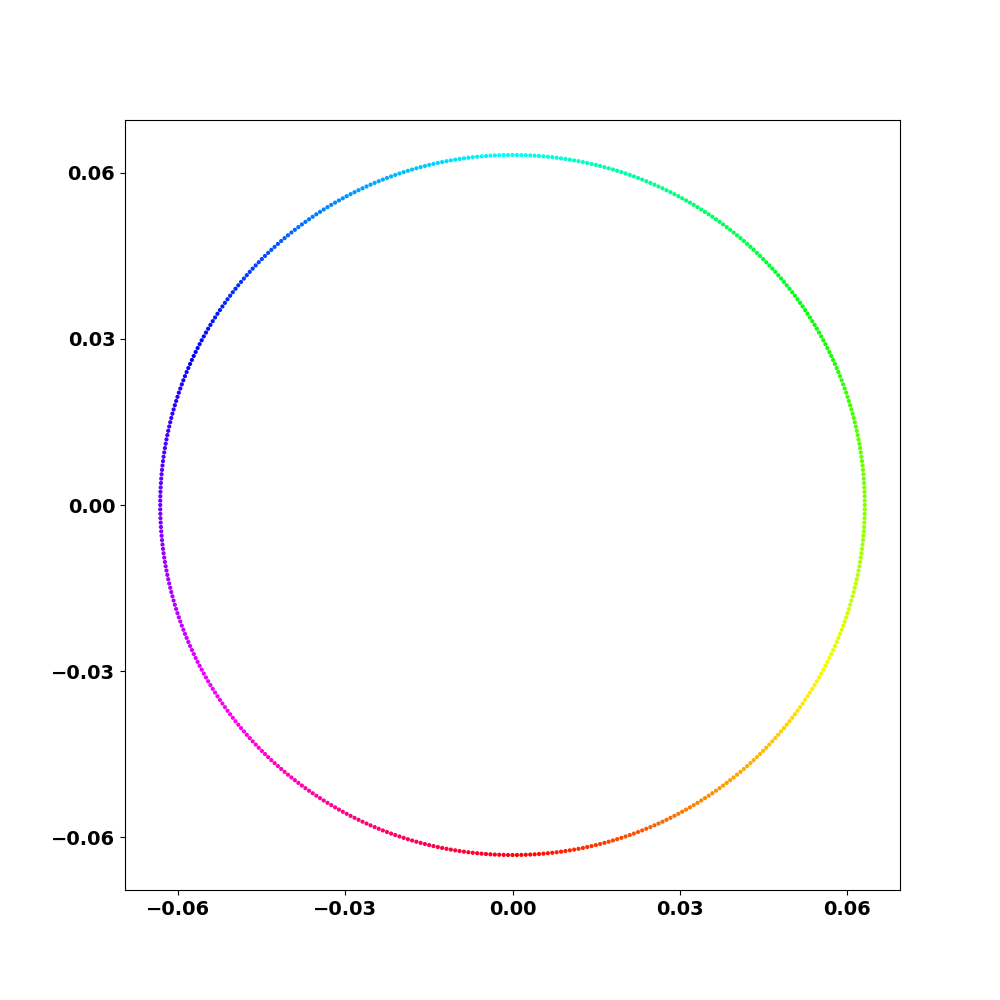
\includegraphics[width=0.8\textwidth]{phaton_clean_manifold.png}
          \caption{GL-Embedding from $k=2$}
      \end{subfigure}\hfill
      \pause
      \begin{subfigure}[t]{0.3\textwidth}
        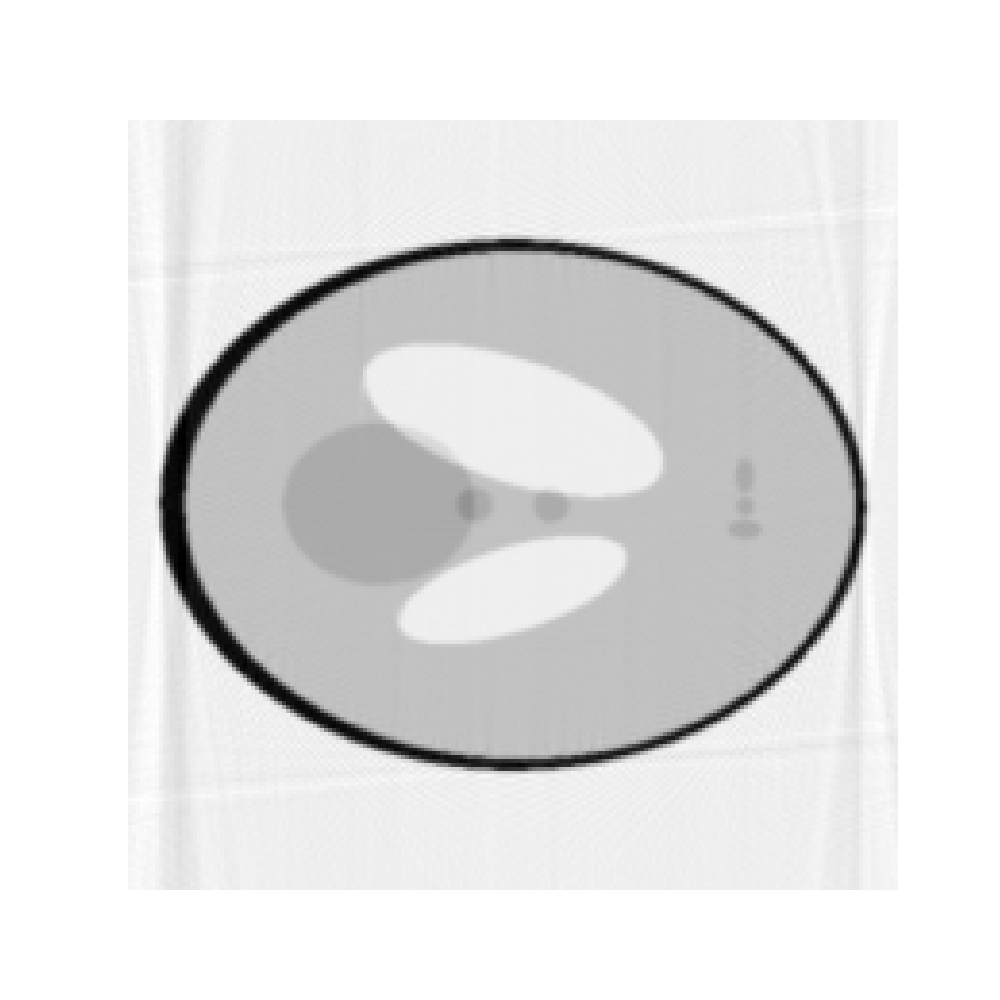
\includegraphics[width=0.8\textwidth]{fbp_phantom_clean_unknown_angles.png}
        \caption{Reconstruction unknown angles}
    \end{subfigure}
    }
    
    \only<4>{
      \begin{subfigure}[t]{0.3\textwidth}
        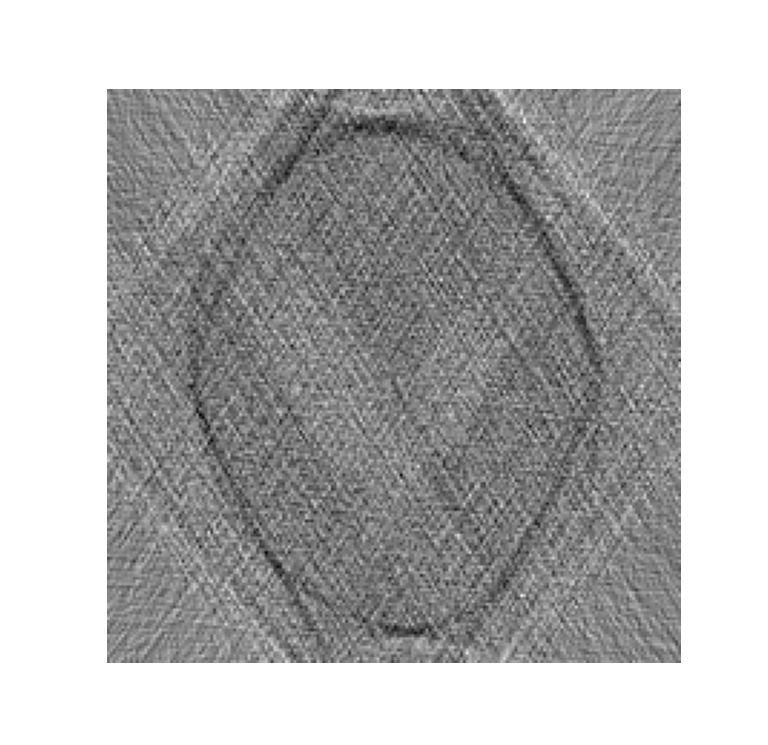
\includegraphics[width=.8\textwidth]{fbp_phantom_snr_0.png}
        \caption{Reconstruction known angles $SNR_y$ : 0 dB}
      \end{subfigure} \hfill
      \begin{subfigure}[t]{0.3\textwidth}
          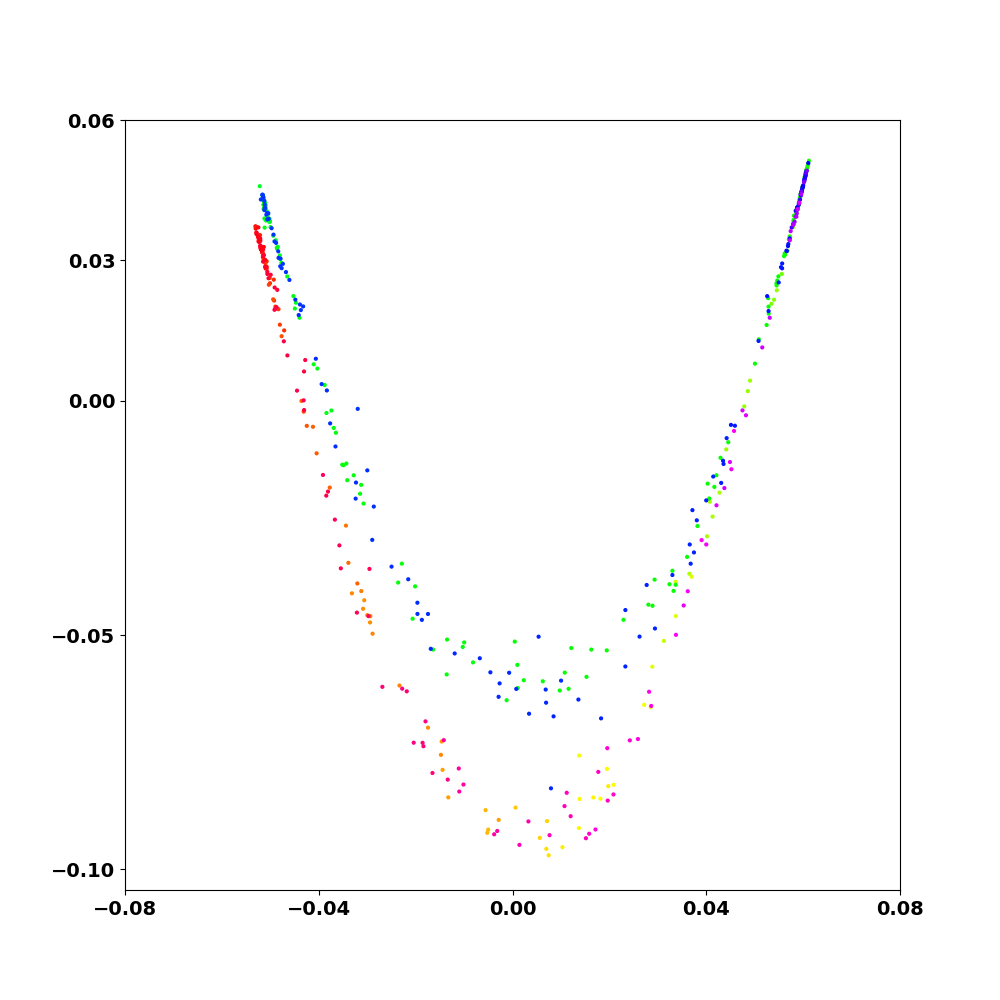
\includegraphics[width=.8\textwidth]{phaton_noisy_manifold_k6_snr0.png}
          \caption{GL-Embedding from $k=6$ and $SNR_y$ : 0 dB }
      \end{subfigure}\hfill
      \begin{subfigure}[t]{0.3\textwidth}
        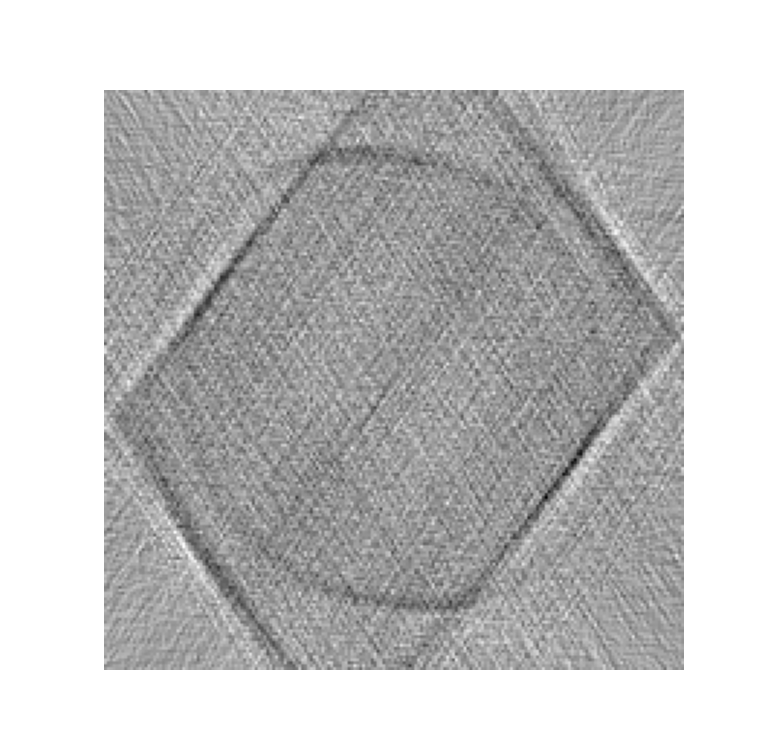
\includegraphics[width=.8\textwidth]{fbp_phantom_snr_0_unknown_angels.png}
        \caption{Reconstruction unknown angles $SNR_y$ : 0 dB}
      \end{subfigure}
    }
  \end{figure}

\end{frame}



\begin{frame}[c]{Graph Denoising}
    \textit{Graph denoising} is the task, to estimate a graph $\tilde{G}$  
    from a given noisy graph $G_0$, with underlying original graph $G$:

    \begin{definition}[Graph Denoising]
        $$GD: G_0 \mapsto \tilde{G} \approx G,$$
    \end{definition}
    where $G_0$, $\tilde{G}$, $G$ denotes noisy, estimated denoised and original graph respectively.
\end{frame}

\begin{frame}{Observation Denoising}

  \begin{itemize}
    \item Use existing denoising algorithms
    \begin{itemize}
      \item Block-matching and 3D filtering (BM3D) \cite{bm3d}
      \item Non-local means \cite{noneLocalMean}
      \item No graph as data structure
      \item But, both exploit neighborhood during averaging.
    \end{itemize}
    \item Show potential for graph as a data structure.
  \end{itemize}

  \begin{tcolorbox}[colback=red!5!white,hide=<-1>, alert=<2>, colframe=red!75!black]
    This is the methodology to approach.
\end{tcolorbox}

  
\end{frame}


\section{GAT-Denoiser}

\begin{frame}{GAT-Denoiser}
  \begin{itemize}
    \item GAT-Denoiser is a graph neural network (GNN) to denoise observations.
    \item Consists of three components:
    \begin{itemize}
      \item \alert<3-4>{Convolution}
      \only<4>{
        \begin{itemize}
          \item \alert{Denoise single observation}
        \end{itemize}
      }
      \item \alert<3-4>{Graph Attention Network (GAT) \cite{GAT}}
      \only<4>{
        \begin{itemize}
          \item \alert{Denoise neighboring  observation}
        \end{itemize}
      }
      
      \item \alert<5-6>{End-to-End Learning}
      \only<5-6>{
        \begin{itemize}
          \item<6> \alert{Optimize for reconstruction quality}
          \item<6> \alert{Loss: $\mathcal{L}_{reconstruction} = \parallel x - \textit{Recon} ( \textit{GAT-Denoiser}(y)) \parallel ^2_2$}
        \end{itemize}
      }
      
    \end{itemize}
  \end{itemize}
  

    \only<2>{
      \begin{figure}
        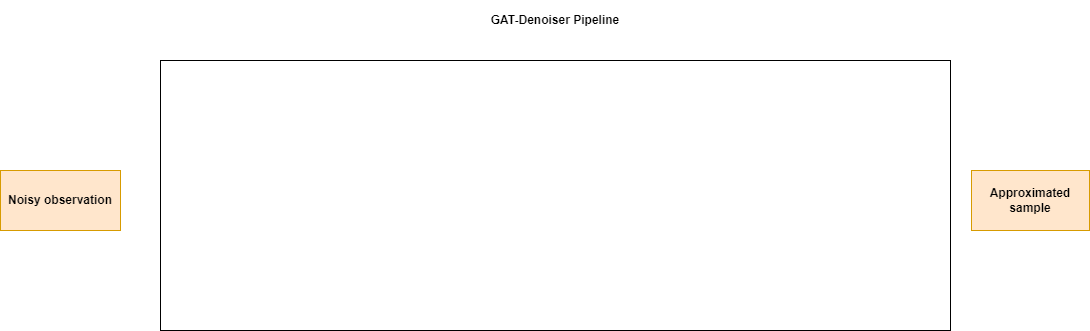
\includegraphics[width=.9\textwidth]{Overall_GAT-Denoiser_Pipeline_3.drawio.png}
      \end{figure}
    }

    \only<3-4>{
      \begin{figure}
        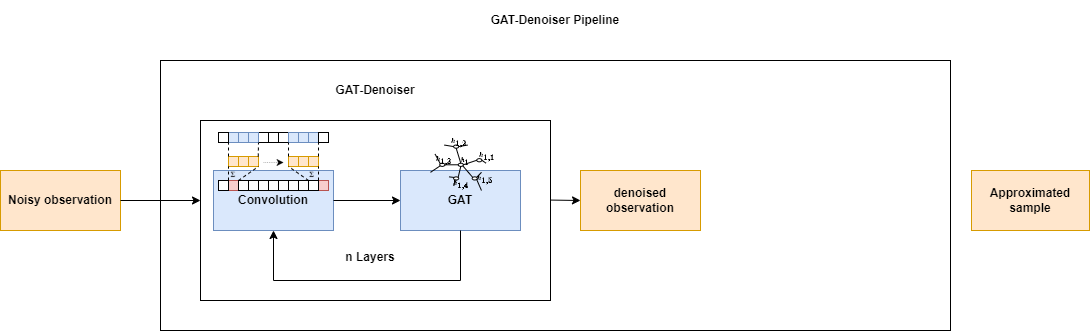
\includegraphics[width=.8\textwidth]{Overall_GAT-Denoiser_Pipeline_2.drawio.png}
      \end{figure}
    }

    \only<5-6>{
      \begin{figure}
        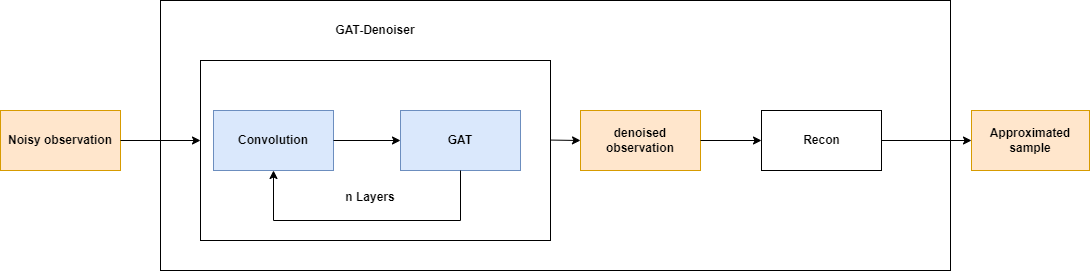
\includegraphics[width=.8\textwidth]{Overall_GAT-Denoiser_Pipeline.drawio.png}
      \end{figure}
    }

      
\end{frame}

% \begin{frame}{GAT-Denoiser Components}
    
%   \begin{itemize}
%     \item<2-> Convolution
%     \begin{itemize}
%       \item Denoise single observation
%     \end{itemize}

%     \item<3-> Graph Attention Network (GAT) \cite{GAT}
%     \begin{itemize}
%       \item Denoise neighboring  observation
%     \end{itemize}
%     \item<4-> End-to-End Learning
%     \begin{itemize}
%       \item Optimize for reconstruction quality
%       \item Loss: $\mathcal{L}_{reconstruction} = \parallel x - \textit{Recon} ( \textit{GAT-Denoiser}(y)) \parallel ^2_2$
      
%     \end{itemize}
%   \end{itemize}

% \end{frame}

\begin{frame}{Graph Attention Network - GAT}
  \pause
  \begin{columns}
  \column{0.6\textwidth}
    \begin{itemize}
      \item Extends Graph Convolution Network with attention (weights)
      \item Computes new node features
      \item Averages graph over neighborhood
      \item Multi-head available, motivated by \cite{transformer}
      \item<3> \alert<3>{$\sigma$: activation function (Exponential Linear Unit)}
      \item<3> \alert<3>{$W$: learnable weight matrix}
      \item<3> \alert<3>{$\alpha$: normalized attention coefficients}
    \end{itemize}
    \column{0.4\textwidth}
    \only<3>{
    \begin{figure}
      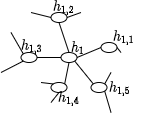
\includegraphics[width=.6\textwidth]{GAT.drawio.png}
    \end{figure}
      $$h_{1}^{\prime} = \sigma \left( \sum_{i=1}^6\alpha_i W h_{i} \right)$$
    }
    
  \end{columns}

\end{frame}


\begin{frame}{Input Graph}
  \pause
  \begin{columns}
    \column{0.6\textwidth}
    \begin{itemize}
      \item Exploit information from GL
      \begin{itemize}
        \item Low-dimensional embedding estimates angles
        \item Dominant information in data can be considered observation angles.
      \end{itemize}
      \item<3-> \alert<3>{Construct graph from observation angles}
      \begin{itemize}
        \item<4-> Map angles to unit-circle / unit-sphere
        \item<5-> Apply k-NN with great-circle distance
      \end{itemize}
    \end{itemize}
    \column{0.4\textwidth}

    \only<4>{
      \begin{figure}
        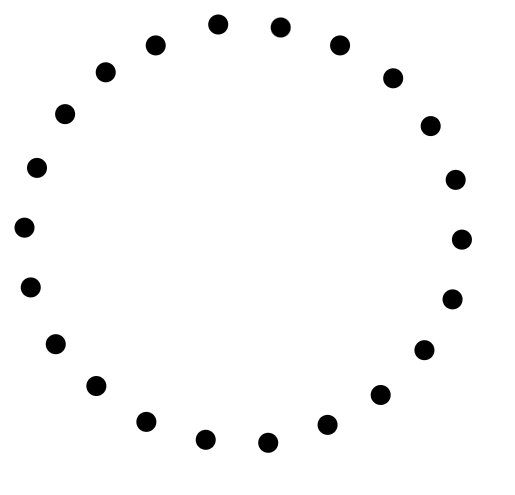
\includegraphics[width=.7\textwidth]{Circle_graph.drawio.png}
      \end{figure}
    }

    \only<5->{
      \begin{figure}
        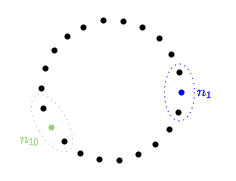
\includegraphics[width=.85\textwidth]{Circle_graphneighbours.drawio.png}
      \end{figure}
    }
    
  \end{columns}
  

  \begin{tcolorbox}[colback=red!5!white,hide=<1-5>, alert=<6>, colframe=red!75!black]
    Observation angles $\theta$ are assumed to be equally spaced on the unit-circle.
\end{tcolorbox}
\end{frame}



\section{Results on LoDoPaB-CT dataset}
% https://latexdraw.com/bar-charts-in-latex-step-by-step-tikz-tutorial/
\begin{frame}{Some result testing}
    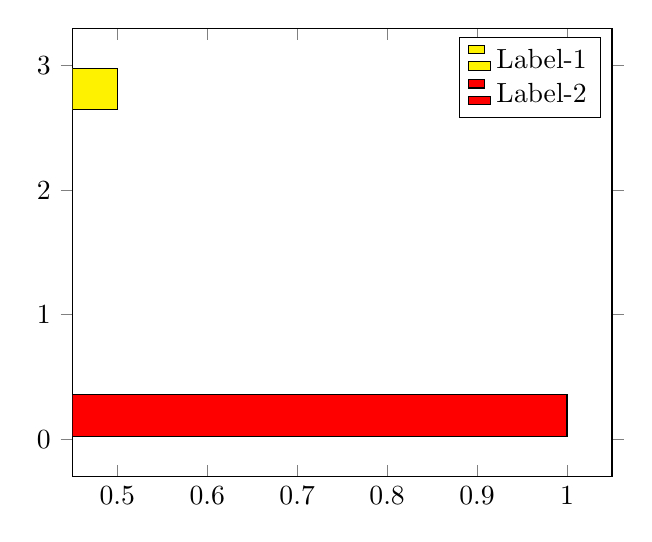
\begin{tikzpicture}
 
        \begin{axis} [xbar,bar width=15pt]
        \addplot[fill = yellow] coordinates { (0.5,3) };
        \addplot[fill = red] coordinates { (1,0) };
        \legend {Label-1, Label-2};
        \end{axis}
         
        \end{tikzpicture}
         

\end{frame}


\section{Summary \& Future Work}

\begin{frame}{Summary}
  \begin{itemize}
    \item GAT-Denoiser enables denoising of observations
    \begin{itemize}
      \item Convolution
      \item GAT
      \item End-To-End Learning
      \item Joint U-Net training boost performance
    \end{itemize}
    \item<2> Evaluated on LoDoPaB-CT dataset
    \begin{itemize}
      \item Outperformed baseline BM3D by up to 379.9 \%
    \end{itemize}
  \end{itemize}
\end{frame}

\begin{frame}{Future Work}

  \begin{itemize}
    \item Improve current GAT-Denoiser
    \item Derive GAT-Denoiser for 3D
    \item Make it work for unknown angles
    \item<2> Cryo-EM
    \begin{itemize}
      \item Known angles
      \item Unknown angles
      \item Work with structural variety in observations
    \end{itemize}
  \end{itemize}

\end{frame}

\section{Questions}
\begin{frame}[c]{Questions}
  \begin{figure}
    \centering
    
\includegraphics[width=0.8\textwidth]{questions.jpg}
  \end{figure}
\end{frame}






\backupbegin

\begin{frame}{References}
    \printbibliography
\end{frame}

\backupend

\end{document}

